% author:   sam tenka
% change:   2022-06-29
% create:   2022-06-29

%==============================================================================
%====  0.  DOCUMENT SETTINGS  ================================================
%==============================================================================

%~~~~~~~~~~~~~~~~~~~~~~~~~~~~~~~~~~~~~~~~~~~~~~~~~~~~~~~~~~~~~~~~~~~~~~~~~~~~~~
%~~~~~~~~~~~~~  0.0. About this Exposition  ~~~~~~~~~~~~~~~~~~~~~~~~~~~~~~~~~~~

%---------------------  0.0.0. page geometry  ---------------------------------
\documentclass[11pt, justified]{tufte-book}
\geometry{
  left           = 0.90in, % left margin
  textwidth      = 4.95in, % main text block
  marginparsep   = 0.15in, % gutter between main text block and margin notes
  marginparwidth = 2.30in, % width of margin notes
                 % 0.20in  % width from margin to edge
}

%---------------------  0.0.1. math packages  ---------------------------------
\newcommand\hmmax{0} % to allow for more fonts 
\newcommand\bmmax{0} % to allow for more fonts
\usepackage{amsmath, amssymb, amsthm, mathtools}
\usepackage{bm}
\usepackage{euler}

\usepackage{array}   % for \newcolumntype macro
\newcolumntype{L}{>{$}l<{$}} % math-mode version of "l" column type
\newcolumntype{C}{>{$}c<{$}} % math-mode version of "c" column type
\newcolumntype{R}{>{$}r<{$}} % math-mode version of "r" column type

%---------------------  0.0.2. graphics packages  -----------------------------
\usepackage{graphicx, xcolor}
\usepackage{float, capt-of}

%---------------------  0.0.3. packages for fancy text  -----------------------
\usepackage{enumitem}\setlist{nosep}
\usepackage{listings}
\usepackage{xstring}
\usepackage{fontawesome5}

%---------------------  0.043. colors  ----------------------------------------
\definecolor{mblu}{rgb}{0.05, 0.35, 0.70} \newcommand{\blu}{\color{mblu}}
\definecolor{mbre}{rgb}{0.30, 0.45, 0.60} \newcommand{\bre}{\color{mbre}}
\definecolor{mbro}{rgb}{0.60, 0.05, 0.05} \newcommand{\bro}{\color{mbro}}
\definecolor{mcya}{rgb}{0.10, 0.45, 0.45} \newcommand{\cya}{\color{mcya}}
\definecolor{mgre}{rgb}{0.55, 0.55, 0.50} \newcommand{\gre}{\color{mgre}}
\definecolor{mgrn}{rgb}{0.15, 0.65, 0.05} \newcommand{\grn}{\color{mgrn}}
\definecolor{mred}{rgb}{0.90, 0.05, 0.05} \newcommand{\red}{\color{mred}}

%~~~~~~~~~~~~~~~~~~~~~~~~~~~~~~~~~~~~~~~~~~~~~~~~~~~~~~~~~~~~~~~~~~~~~~~~~~~~~~
%~~~~~~~~~~~~~  0.1. Headers and References  ~~~~~~~~~~~~~~~~~~~~~~~~~~~~~~~~~~

%---------------------  0.1.0. intra-document references  ---------------------
\newcommand{\offour}[1]{
    {\tiny \raisebox{0.04cm}{\scalebox{0.9}{$\substack{
        \IfSubStr{#1}{0}{{\blacksquare}}{\square}   
        \IfSubStr{#1}{1}{{\blacksquare}}{\square} \\ 
        \IfSubStr{#1}{2}{{\blacksquare}}{\square}   
        \IfSubStr{#1}{3}{{\blacksquare}}{\square}   
    }$}}}%
}

\newcommand{\offourline}[1]{
    {\tiny \raisebox{0.04cm}{\scalebox{0.9}{$\substack{
        \IfSubStr{#1}{0}{{\blacksquare}}{\square}   
        \IfSubStr{#1}{1}{{\blacksquare}}{\square}
        \IfSubStr{#1}{2}{{\blacksquare}}{\square}   
        \IfSubStr{#1}{3}{{\blacksquare}}{\square}   
    }$}}}%
}
\newcommand{\notesam}[1]{{\blu \textsf{#1}}}
\newcommand{\attn}[1]{{\bro \textsf{#1}}}
\newcommand{\attnsam}[1]{{\red \textsf{#1}}}

\newcommand{\blarr}{\hspace{-0.15cm}${\bro \leftarrow}\,$}
\newcommand{\bcirc}{${\bro ^\circ}$}

%---------------------  0.1.1. table of contents helpers  ---------------------
\newcommand{\phdot}{\phantom{.}}

%---------------------  0.1.2. section headers  -------------------------------
\newcommand{\samtitle} [1]{
  \par\noindent{\Huge \sf \blu #1}
  \vspace{0.4cm}
}

\newcommand{\samquote} [2]{
    \marginnote[-0.4cm]{\begin{flushright}
    \scriptsize
        \gre {\it #1} \\ --- #2
    \end{flushright}}
}

\newcommand{\samsection} [1]{
  \vspace{0.5cm}
  \par\noindent{\LARGE \sf \blu #1}
  \vspace{0.1cm}\par
}

\newcommand{\samsubsection}[1]{
  \vspace{0.3cm}
  \par\noindent{\Large \sf \bre #1}
  \vspace{0.1cm}\par
}

\newcommand{\samsubsubsection}[1]{
   \vspace{0.1cm}
   \par\noindent{\hspace{-2cm}\normalsize \sc \gre #1} ---
}

%---------------------  0.1.3. clear the bibliography's header  ---------------
\usepackage{etoolbox}
\patchcmd{\thebibliography}{\section*{\refname}}{}{}{}

%~~~~~~~~~~~~~~~~~~~~~~~~~~~~~~~~~~~~~~~~~~~~~~~~~~~~~~~~~~~~~~~~~~~~~~~~~~~~~~
%~~~~~~~~~~~~~  0.2. Math Symbols and Blocks  ~~~~~~~~~~~~~~~~~~~~~~~~~~~~~~~~~

%---------------------  0.2.0. general math operators  ------------------------
\newcommand{\scirc}{\mathrel{\mathsmaller{\mathsmaller{\mathsmaller{\circ}}}}}
\newcommand{\cmop}[2]{{(#1\!\to\!#2)}}

%---------------------  0.2.1. probability symbols  ---------------------------
\newcommand{\KL}{\text{KL}}
\newcommand{\EN}{\text{H}}
\newcommand{\note}[1]{{\blu \textsf{#1}}}

%---------------------  0.2.2. losses averaged in various ways  ---------------
\newcommand{\Ein}  {\text{trn}_{\sS}}
\newcommand{\Einb} {\text{trn}_{\check\sS}}
\newcommand{\Einc} {\text{trn}_{\sS\sqcup \check\sS}}
\newcommand{\Egap} {\text{gap}_{\sS}}
\newcommand{\Eout} {\text{tst}}

%---------------------  0.2.3. double-struck and caligraphic upper letters  ---
\newcommand{\Aa}{\mathbb{A}}\newcommand{\aA}{\mathcal{A}}
\newcommand{\Bb}{\mathbb{B}}\newcommand{\bB}{\mathcal{B}}
\newcommand{\Cc}{\mathbb{C}}\newcommand{\cC}{\mathcal{C}}
\newcommand{\Dd}{\mathbb{D}}\newcommand{\dD}{\mathcal{D}}
\newcommand{\Ee}{\mathbb{E}}\newcommand{\eE}{\mathcal{E}}
\newcommand{\Ff}{\mathbb{F}}\newcommand{\fF}{\mathcal{F}}
\newcommand{\Gg}{\mathbb{G}}\newcommand{\gG}{\mathcal{G}}
\newcommand{\Hh}{\mathbb{H}}\newcommand{\hH}{\mathcal{H}}
\newcommand{\Ii}{\mathbb{I}}\newcommand{\iI}{\mathcal{I}}
\newcommand{\Jj}{\mathbb{J}}\newcommand{\jJ}{\mathcal{J}}
\newcommand{\Kk}{\mathbb{K}}\newcommand{\kK}{\mathcal{K}}
\newcommand{\Ll}{\mathbb{L}}\newcommand{\lL}{\mathcal{L}}
\newcommand{\Mm}{\mathbb{M}}\newcommand{\mM}{\mathcal{M}}
\newcommand{\Nn}{\mathbb{N}}\newcommand{\nN}{\mathcal{N}}
\newcommand{\Oo}{\mathbb{O}}\newcommand{\oO}{\mathcal{O}}
\newcommand{\Pp}{\mathbb{P}}\newcommand{\pP}{\mathcal{P}}
\newcommand{\Qq}{\mathbb{Q}}\newcommand{\qQ}{\mathcal{Q}}
\newcommand{\Rr}{\mathbb{R}}\newcommand{\rR}{\mathcal{R}}
\newcommand{\Ss}{\mathbb{S}}\newcommand{\sS}{\mathcal{S}}
\newcommand{\Tt}{\mathbb{T}}\newcommand{\tT}{\mathcal{T}}
\newcommand{\Uu}{\mathbb{U}}\newcommand{\uU}{\mathcal{U}}
\newcommand{\Vv}{\mathbb{V}}\newcommand{\vV}{\mathcal{V}}
\newcommand{\Ww}{\mathbb{W}}\newcommand{\wW}{\mathcal{W}}
\newcommand{\Xx}{\mathbb{X}}\newcommand{\xX}{\mathcal{X}}
\newcommand{\Yy}{\mathbb{Y}}\newcommand{\yY}{\mathcal{Y}}
\newcommand{\Zz}{\mathbb{Z}}\newcommand{\zZ}{\mathcal{Z}}

%---------------------  0.2.4. sans serif and frak lower letters  -------------
\newcommand{\sfa}{\mathsf{a}}\newcommand{\fra}{\mathcal{a}}
\newcommand{\sfb}{\mathsf{b}}\newcommand{\frb}{\mathcal{b}}
\newcommand{\sfc}{\mathsf{c}}\newcommand{\frc}{\mathcal{c}}
\newcommand{\sfd}{\mathsf{d}}\newcommand{\frd}{\mathcal{d}}
\newcommand{\sfe}{\mathsf{e}}\newcommand{\fre}{\mathcal{e}}
\newcommand{\sff}{\mathsf{f}}\newcommand{\frf}{\mathcal{f}}
\newcommand{\sfg}{\mathsf{g}}\newcommand{\frg}{\mathcal{g}}
\newcommand{\sfh}{\mathsf{h}}\newcommand{\frh}{\mathcal{h}}
\newcommand{\sfi}{\mathsf{i}}\newcommand{\fri}{\mathcal{i}}
\newcommand{\sfj}{\mathsf{j}}\newcommand{\frj}{\mathcal{j}}
\newcommand{\sfk}{\mathsf{k}}\newcommand{\frk}{\mathcal{k}}
\newcommand{\sfl}{\mathsf{l}}\newcommand{\frl}{\mathcal{l}}
\newcommand{\sfm}{\mathsf{m}}\newcommand{\frm}{\mathcal{m}}
\newcommand{\sfn}{\mathsf{n}}\newcommand{\frn}{\mathcal{n}}
\newcommand{\sfo}{\mathsf{o}}\newcommand{\fro}{\mathcal{o}}
\newcommand{\sfp}{\mathsf{p}}\newcommand{\frp}{\mathcal{p}}
\newcommand{\sfq}{\mathsf{q}}\newcommand{\frq}{\mathcal{q}}
\newcommand{\sfr}{\mathsf{r}}\newcommand{\frr}{\mathcal{r}}
\newcommand{\sfs}{\mathsf{s}}\newcommand{\frs}{\mathcal{s}}
\newcommand{\sft}{\mathsf{t}}\newcommand{\frt}{\mathcal{t}}
\newcommand{\sfu}{\mathsf{u}}\newcommand{\fru}{\mathcal{u}}
\newcommand{\sfv}{\mathsf{v}}\newcommand{\frv}{\mathcal{v}}
\newcommand{\sfw}{\mathsf{w}}\newcommand{\frw}{\mathcal{w}}
\newcommand{\sfx}{\mathsf{x}}\newcommand{\frx}{\mathcal{x}}
\newcommand{\sfy}{\mathsf{y}}\newcommand{\fry}{\mathcal{y}}
\newcommand{\sfz}{\mathsf{z}}\newcommand{\frz}{\mathcal{z}}

%---------------------  0.2.5. math environments  -----------------------------
\newtheorem*{qst}{Question}
\newtheorem*{thm}{Theorem}
\newtheorem*{lem}{Lemma}
% ...
\theoremstyle{definition}
\newtheorem*{dfn}{Definition}

%==============================================================================
%=====  1.  DOCUMENT PROPER  ==================================================
%==============================================================================

\begin{document}

  \newcommand{\rowzero}{\textsc{Philip,  Mariana, Mawuko}}
  \newcommand{\rowone }{\textsc{James,   Bereket, Amadeo}}
  %
  \newcommand{\cola}   {\textsc{Philip,  James}}
  \newcommand{\colb}   {\textsc{Mariana, Bereket}}
  \newcommand{\colc}   {\textsc{Mawuko,  Amadeo}}
  %
  \newcommand{\exercise}[2]{\par\noindent\attn{Exercise} (#1): \emph{#2}}
  %\newcommand{\exercise}[2]{\marginnote{\attn{Exercise} (#1): \emph{#2}}}

%~~~~~~~~~~~~~~~~~~~~~~~~~~~~~~~~~~~~~~~~~~~~~~~~~~~~~~~~~~~~~~~~~~~~~~~~~~~~~~
%~~~~~~~~~~~~~  1.0. front matter  ~~~~~~~~~~~~~~~~~~~~~~~~~~~~~~~~~~~~~~~~~~~~

  \samtitle{recitation 06 (optional 6.86x notes)}

  \noindent
    Let's start NEURAL NETWORKS!  Hurrah!
    By today's end, we'll be able to: 
    \begin{description}
        %\item[\hspace{1cm}] \emph{contrast} with kernel 
        %\item[\hspace{1cm}] \emph{reason about} convexity of learning 
        \item[\hspace{1cm}] \emph{implement} training and prediction code for
                            a shallow neural classifier
        \item[\hspace{1cm}] \emph{compute} gradient updates for shallow and deep neural
                            networks 
        \item[\hspace{1cm}] \emph{diagnose} and remedy bad initialization
                            widths and learning rates
    \end{description}
    Our rough schedule is:
    \begin{description}
        \item[\hspace{1cm}] \emph{19:30} what's a neural network? 
        \item[\hspace{1cm}] \emph{19:45} which features are most helpful? --- math problems
        \item[\hspace{1cm}] \emph{20:00} making features better --- math problems
        \item[\hspace{1cm}] \emph{20:15} making features better --- code problems
        \item[\hspace{1cm}] \emph{20:30} what happens during training? --- visual example
        \item[\hspace{1cm}] \emph{20:45} how do design decisions affect error? 
        \item[\hspace{1cm}] \emph{21:00}  
    \end{description}
    As always, \attn{please ask questions} at any time, including by
    interrupting me!

  \samsection{C. automatic featurization}

%~~~~~~~~~~~~~~~~~~~~~~~~~~~~~~~~~~~~~~~~~~~~~~~~~~~~~~~~~~~~~~~~~~~~~~~~~~~~~~
%~~~~~~~~~~~~~  1.1. ~~~~~~~~~~~~~~~~~~~~~~~~~~~~~~~~~~~~~~~~~~~~~~~~~~~~~~~~~~

    \samsubsection{new features from old}%automatic featurization}

      \samsubsubsection{architecture and expressivity}
        Last week, we saw how approximation and generalization depend crucially
        on how we \emph{featurize} our data.  We made our models more
        expressive by nonlinearly transforming our `raw' features into the
        features on which we actually do linear classification.
        %
        Last week, we nonlinearly transformed according to hand-designed
        functions such as a quadratic.  Today, we'll reduce the amount of
        manual labor by \emph{fitting} a nonlinear `featurizer function' to
        data!
        %
        There are two conceptual components here: first, we've got to
        parameterize a family of possible featurizers (that's part of
        \textbf{architecture}) and second, we've got to figure out how to find
        a good featurizer from among this family.

        First, architecture.\marginnote{%
          We define the \textbf{relu} function by\vspace{-0.1cm}
          $$
            \text{relu}(z) = \max(0,z) \vspace{-0.1cm}
          $$
          Do you see what this looks like?
        }
        We'll define a bunch of features $h_j$
        by $h_j=\text{relu}(\sum_i A_{ji} x_i)$.  The $A_{ji}$s
        are parameters to figure out.  This model is a \textbf{shallow
        neural net}.

        \begin{figure}[h]
          \centering
            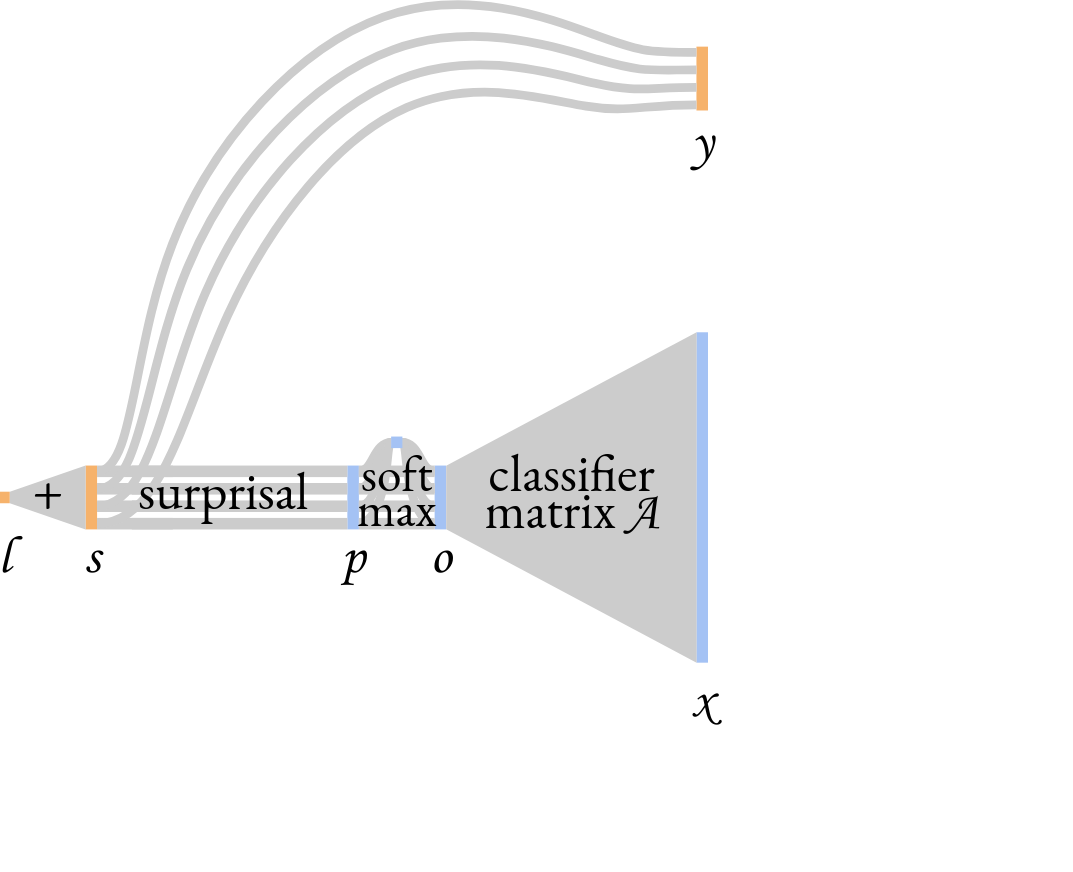
\includegraphics[width=0.468\textwidth]{linear}
            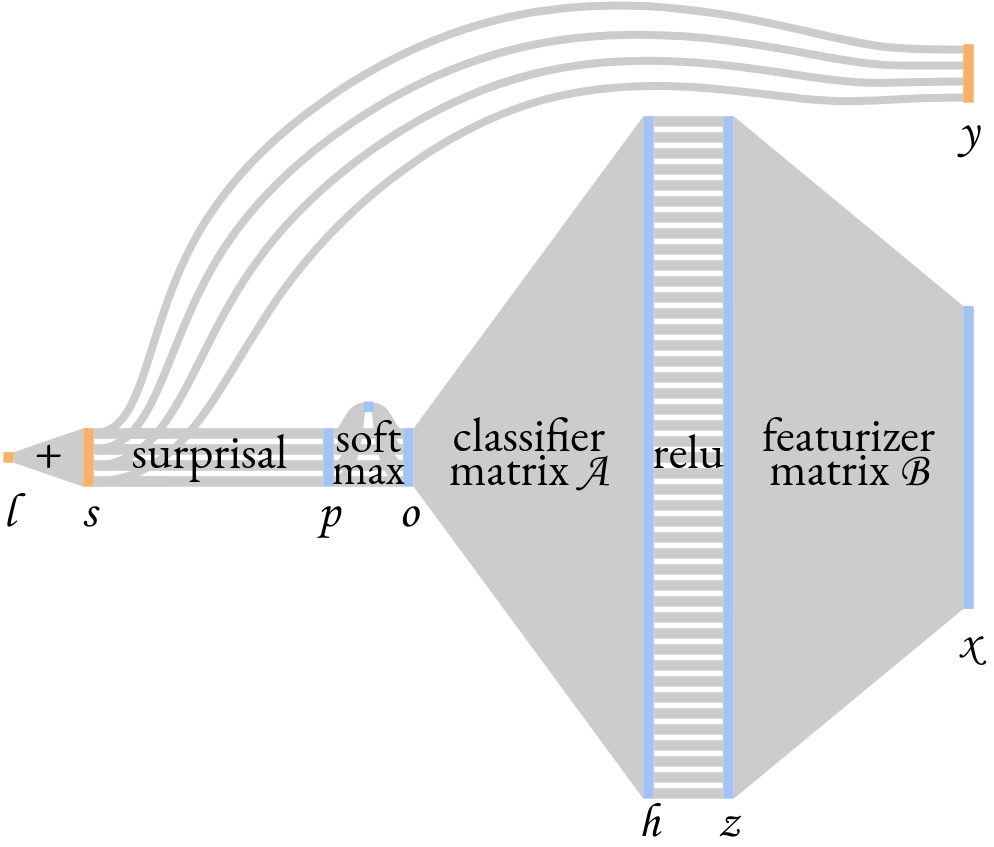
\includegraphics[width=0.423\textwidth]{shallow}
          \caption{%
            \textbf{Linear models (left) vs shallow neural nets (right).}
            Data flows right to left via {\gre gray} transforms.  The thin
            vertical strips depict vectors; the small squares, scalars.  We use
            the {\blu blue} quantities to predict.  We additionally use
            {\color{orange} orange} to learn from data.
            %
            Both models use maximum likelihood loss on softmax
            predictions:\vspace{-0.1cm}
            %
            $$
                \ell = \textstyle\sum_k s_k 
                \quad
                s_k = y_k \log(1/p_k)
            $$
            \vspace{-0.4cm}
            $$
                p_k = \exp(o_k) /\!\textstyle\sum_{\tilde k} \exp(o_{\tilde k})
            $$
            %
            The models both set the decision function $o$ as a linear
            combination of ``features'' but the two differ in how they compute
            those features.  The linear model (left) simply uses the raw input
            features $x$; the shallow neural net (right) uses features $h$
            nonlinearly transformed from $x$:\vspace{-0.1cm}
            $$
                o_k = \textstyle\sum_{i} A_{ki} x_i 
                \quad
                \text{OR}
                \quad
                o_k = \textstyle\sum_{j} A_{kj} h_j 
            $$
            Each ``\textbf{hidden activation}'' or 
            ``\textbf{learned feature}'' $h_j$ measures tresspass past a linear
            boundary determined by a matrix $B$:\vspace{-0.1cm}
            $$
                h_j = \text{relu}(z_j)
                \quad
                z_j = \textstyle\sum_{i} B_{ji} x_i 
            $$
          }
        \end{figure}

        \exercise{\rowzero}{if our featurizer matrix $B$ has shape $10\times 3$,
        and if there are $4$ labels, then what shape is the classifier matrix $A$?}

        \pagebreak
        \begin{marginfigure}%[h]%
          \centering
          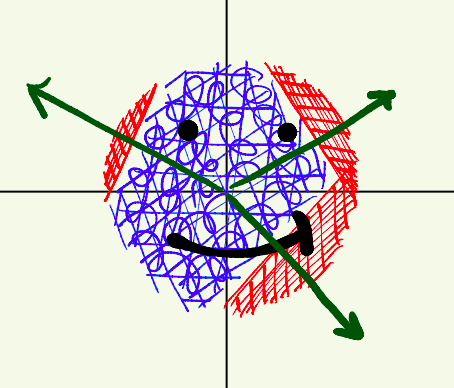
\includegraphics[width=0.4445\textwidth]{smiley}%
          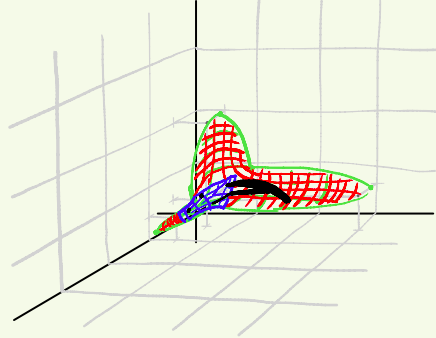
\includegraphics[width=0.49\textwidth]{smiley-transformed}%
            \caption{\textbf{Smiley Data.} \textbf{Left.} Our 2D raw input
            vectors with binary class labels in red and blue.  The black and
            green marks are merely annotations.  \textbf{Right.} The smiley
            data transformed according to a $B$ matrix whose rows are given by
            the three green arrows.  To aid visualization, we used a variant
            of relu, namely $f(z) = \max(\exp(-z),1+z)$}
        \end{marginfigure}
        %\begin{figure}%
        %  \centering
        %  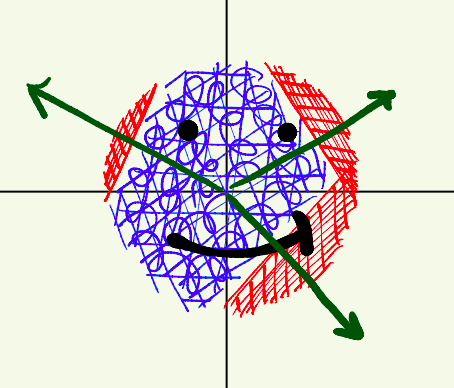
\includegraphics[width=0.49\textwidth]{smiley}%
        %\end{figure}
        Which models can exactly fit the smiley data in the margin?  (Imagine a
        very very thin unpopulated boundary between red and blue; lines that
        appear straight-ish are supposed to be exactly straight.) 
        %
        \exercise{\colc}{...a quadratic ($6$-feature) kernel svm?}
        %
        \exercise{\cola}{...a cubic ($10$-feature) kernel svm?}
        %
        \exercise{\colb}{...a shallow neural network with $4$ learned features?}
        %\begin{marginfigure}%
        %  \centering
        %  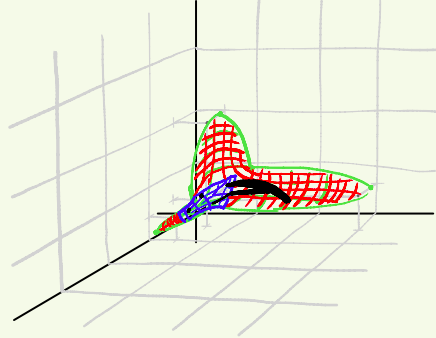
\includegraphics[width=0.99\textwidth]{smiley-transformed}%
        %\end{marginfigure}

      \samsubsubsection{training with random fixed features}
        To further fortify our intuition for these new features, let's randomly
        set $B$ and see how linear classification works on the resulting new
        features.  We'll work with this artificial galaxy dataset for ease of
        visualization:
        \exercise{\rowone} {which features look most useful?}

      \samsubsubsection{sensitivity analysis}

        \exercise{\rowone} {what's a formula for $\partial \ell / \partial
        o_k$?}
        %
        \exercise{\rowzero}{what's a formula for $\partial \ell / \partial
        h_j$?}

%~~~~~~~~~~~~~~~~~~~~~~~~~~~~~~~~~~~~~~~~~~~~~~~~~~~~~~~~~~~~~~~~~~~~~~~~~~~~~~
%~~~~~~~~~~~~~  1.2. ~~~~~~~~~~~~~~~~~~~~~~~~~~~~~~~~~~~~~~~~~~~~~~~~~~~~~~~~~~

    \samsubsection{fitting features to data}
      \samsubsubsection{organizing derivative calculations for gradient descent}

        The following four exercises depend on given weight matrices
        and input data.
        %
        \exercise{\rowone} {what code computes the predicted probability?}
        %
        \exercise{\rowzero}{what code computes $\partial \ell / \partial o_k$?}
        %
        \exercise{\rowzero}{what code computes $\partial \ell / \partial z_j$?}
        %
        \exercise{\rowone} {what code computes $\partial \ell / \partial
        A_{kj}$ and $\partial \ell / \partial B_{ji}$?}

      \samsubsubsection{horizontal vs vertical learning signals}
        In the next three questions\marginnote{%
        To compare likes with likes, we'll fix the raw input featurization and
        use standard softmax throughout; we won't compare different
        kernels to each other.  When we speak of ``different models'', we thus
        mean ``models whose weight matrices (necessarily of the same shapes)
        differ''.  The one weight matrix of a linear model has shape
        $$
            (\text{\# classes} \times \text{\# raw features})
        $$
        The two weight matrices of a shallow neural network have shape
        \begin{align*}
            (\text{\# classes} &\times \text{\# learned features}),\\
            (\text{\# learned features} &\times \text{\# raw features})
        \end{align*}
        } we'll compare various machine learning models.
        %
        \exercise{\cola}{Can different linear models induce the same function
        from inputs to labels?}
        %
        \exercise{\colb}{Can different linear models induce the same function
        from inputs to label probabilities?}
        %
        \exercise{\colc}{Can different shallow neural nets induce the same
        function from inputs to label probabilities?}

        % nonconvexity and symmetry!!!!


%~~~~~~~~~~~~~~~~~~~~~~~~~~~~~~~~~~~~~~~~~~~~~~~~~~~~~~~~~~~~~~~~~~~~~~~~~~~~~~
%~~~~~~~~~~~~~  1.3. ~~~~~~~~~~~~~~~~~~~~~~~~~~~~~~~~~~~~~~~~~~~~~~~~~~~~~~~~~~

    \pagebreak
    \samsubsection{dynamics of shallow net learning}
      \samsubsubsection{visualizing learning dynamics}
        \begin{figure}[h]%
          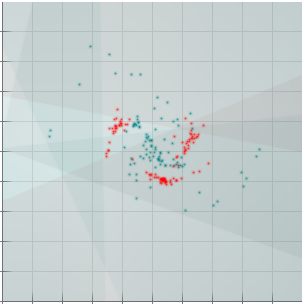
\includegraphics[width=0.199\textwidth]{example-shallow/woah-08-0000}%
          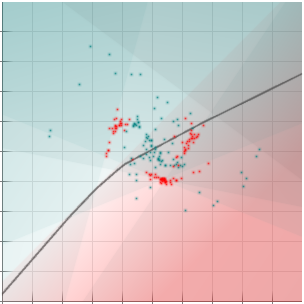
\includegraphics[width=0.199\textwidth]{example-shallow/woah-08-0500}%
          %
          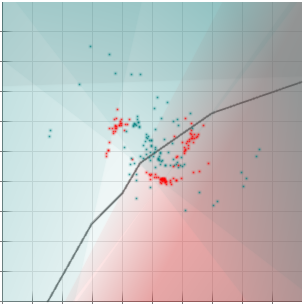
\includegraphics[width=0.199\textwidth]{example-shallow/woah-08-1000}%
          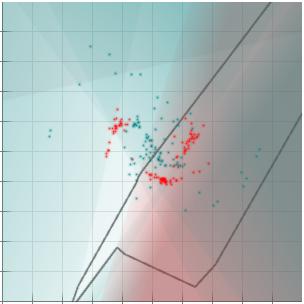
\includegraphics[width=0.199\textwidth]{example-shallow/woah-08-1500}%
          %
          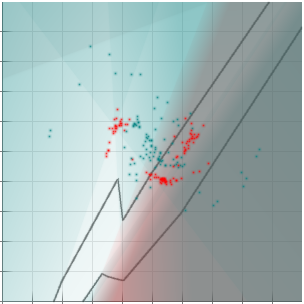
\includegraphics[width=0.199\textwidth]{example-shallow/woah-08-2000}\\%
          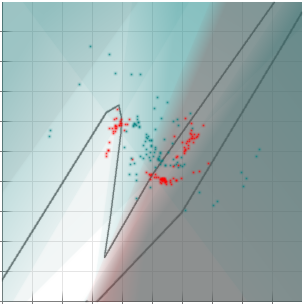
\includegraphics[width=0.199\textwidth]{example-shallow/woah-08-2500}%
          %
          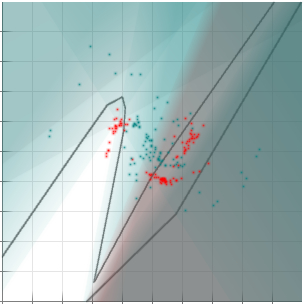
\includegraphics[width=0.199\textwidth]{example-shallow/woah-08-3000}%
          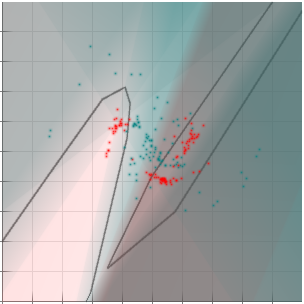
\includegraphics[width=0.199\textwidth]{example-shallow/woah-08-3500}%
          %
          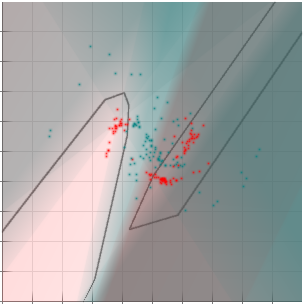
\includegraphics[width=0.199\textwidth]{example-shallow/woah-08-4000}%
          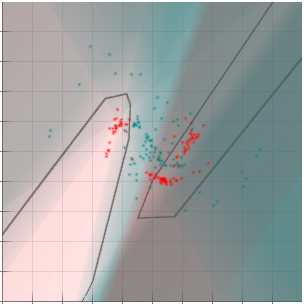
\includegraphics[width=0.199\textwidth]{example-shallow/woah-08-4500}%
        \end{figure}

      \samsubsubsection{initialization and learning rate}
        In the next three questions, we initialize $A=B=0$.  
        %
        \exercise{\colb}{What is the training loss at initialization?}
        %
        \exercise{\colc}{What is the loss gradient at
        initialization?}
        %
        \exercise{\cola}{What is the testing accuracy after a thousand SGD
        updates?}

      \samsubsubsection{hyperparameters affect generalization}

        \exercise{\rowone} {why is the generalization gap usually positive?}
        \exercise{\rowzero}{why not just gradient descend on test loss?}

        For the two questions below, we assume a fixed, smallish training set
        size and a fixed, moderate number of gradient descent steps.
        %
        \exercise{\rowzero}{what should the training and testing accuracies look
                            like as a function of hidden dimension?}
        %
        \exercise{\rowone} {what should the training and testing accuracies look
                            like as a function of the learning rate?}

        % hidden dimension
        % training time
        % regularization of weights
        % dropout

\end{document}

